\documentclass[25pt, a0paper, portrait, blockverticalspace=20mm, innermargin=6mm, titletotopverticalspace=8mm, titletoblockverticalspace=8mm]{tikzposter}

% ==========================================
% CONFIGURACIÓN DE IDIOMA Y PAQUETES
% ==========================================
\usepackage[utf8]{inputenc}
\usepackage[T1]{fontenc}
\usepackage{lmodern}
\usepackage[spanish, provide=*]{babel}
\usepackage{graphicx}
\usepackage[square, numbers, sort&compress]{natbib}
\usepackage{booktabs}
\usepackage{url}
\urlstyle{same}
\usepackage{enumitem}

% ------------------------------------------
% TAMAÑOS DE LETRA
% El póster se diseña en A0 y se imprime en A1 (todo se reduce al 71 %).
%   Texto de las tarjetas: 31 pt en A0  ->  unos 21.9 pt impreso en A1
%   Tablas:                28 pt en A0  ->  unos 19.8 pt impreso en A1
%   Referencias:           26 pt en A0  ->  unos 18.4 pt impreso en A1
% ------------------------------------------
\newcommand{\textoposter}{\fontsize{31pt}{37.2pt}\selectfont}
\newcommand{\textotabla}{\fontsize{28pt}{33.6pt}\selectfont}
\newcommand{\textoreferencias}{\fontsize{26pt}{31.2pt}\selectfont}

\setlength{\bibsep}{0pt plus 0.3ex}
\setlist[itemize]{itemsep=3mm, topsep=3mm, labelsep=0.6em,
  label=\raisebox{0.15ex}{\rule{0.9ex}{0.9ex}}}

% Cifra de pruebas automáticas: se cambia aquí y se actualiza todo el póster.
\newcommand{\pruebasN}{340}

% Figura (imagen o diagrama) con su pie justo debajo. Ocupa su alto natural, y
% lo que falte para llegar al alto del recuadro se guarda en \sobrante para
% repartirlo en la tarjeta. Así la columna mide lo mismo sin importar la
% proporción de la imagen.
% Uso: \figura{alto del recuadro}{contenido}{pie}
\newlength{\sobrante}
\newsavebox{\cajafigura}
\newcommand{\figura}[3]{%
  \sbox{\cajafigura}{\parbox[t]{\linewidth}{\centering
    #2\par
    \vspace{3mm}\raggedright\textit{#3}}}%
  \usebox{\cajafigura}%
  \global\sobrante=\dimexpr #1-\ht\cajafigura-\dp\cajafigura\relax}

% Contenido de una tarjeta centrado a lo alto: el espacio extra se reparte
% mitad arriba y mitad abajo. También escribe en el .log el alto natural.
% Uso: \centrado{espacio extra}{contenido}
\newsavebox{\cajatarjeta}
\newcommand{\centrado}[2]{%
  \sbox{\cajatarjeta}{\parbox[t]{\linewidth}{#2}}%
  \typeout{ALTO-TARJETA: \the\dimexpr\ht\cajatarjeta+\dp\cajatarjeta\relax}%
  \parbox[c][\dimexpr\ht\cajatarjeta+\dp\cajatarjeta+#1\relax][c]{\linewidth}{%
    \usebox{\cajatarjeta}}}

% Separación entre apartados dentro de una tarjeta.
\newcommand{\separa}{\par\vspace{8mm}}

% Los logos son opcionales: si falta el archivo, simplemente no se dibujan.
\newcommand{\logoopcional}[2]{\IfFileExists{#2}{\includegraphics[#1]{#2}}{}}

% Si falta una captura, el póster compila igual con un recuadro.
% Las capturas salen de docs/evidencia-tema-de-color/ del repositorio. Si se
% sube a Overleaf, hay que copiar esa carpeta junto al .tex y ajustar la ruta.
\newcommand{\imagenopcional}[2]{%
  \IfFileExists{#2}{\includegraphics[#1]{#2}}%
  {\fbox{\parbox{0.6\linewidth}{\centering Falta la imagen \texttt{#2}}}}}

% ==========================================
% ESTILO
% ==========================================
\usetheme{Default}
\usetitlestyle{Default}
\useblockstyle{Default}
\setlength{\columnsep}{10mm}

% Los diagramas (arquitectura y flujo de trabajo) se dibujan con el skill
% diagram-design con la paleta de Cabal; sus fuentes HTML y PNG están en
% diagramas/.

% ==========================================
% ENCABEZADO DEL PÓSTER
% ==========================================
\title{\parbox{\linewidth}{\centering {\fontsize{110pt}{120pt}\selectfont\textbf{CABAL}}}}

\author{De León L., Ixcot D., Sac M., Vasquez J. y Méndez A.}
\institute{Universidad Mesoamericana, Sede Quetzaltenango, Facultad de Ingeniería \\ Programación de Dispositivos Móviles, Sección D \\ Noviembre 2026}
\titlegraphic{\logoopcional{height=8cm}{logo1.png} \hspace{2cm} \logoopcional{height=8cm}{logo2.png} \hspace{2cm} \logoopcional{height=8cm}{logo3.png}}

\begin{document}
\maketitle

\begin{columns}

% ==========================================
% COLUMNA 1
% ==========================================
\column{0.33}

\block{INTRODUCCIÓN}{
  \textoposter
  \centrado{150pt}{%
  En las tiendas de colonia de Guatemala, una sola persona atiende, cobra y
  compra la mercadería. \textit{Cabal} es la palabra con que se dice que una
  cuenta sale exacta.

  \separa
  \textbf{Problema}\\
  Los tenderos entrevistados no registran sus ventas o las anotan después de
  memoria, así que compran \guillemotleft a puro cálculo\guillemotright{} y se
  enteran tarde de qué productos no rotan.

  \separa
  \textbf{Objetivo general}\\
  Construir una app móvil sin conexión para que un tendero registre sus ventas
  y vea el cierre del día.

  \separa
  \textbf{Objetivos específicos}
  \begin{itemize}
    \item Validar el problema con entrevistas a tenderos.
    \item Definir una arquitectura en capas con Riverpod y SQLite.
    \item Implementar catálogo, ventas, historial y cierre del día.
    \item Asegurar la calidad con pruebas automáticas y CI.
    \item Dejar escritas las decisiones técnicas y el uso de IA.
  \end{itemize}
  }
}

\block{CITA CLAVE}{
  \textoposter
  \centrado{80pt}{%
  \textit{\guillemotleft Realmente no se lleva ningún control, solo tal vez al
  final contar todo lo que se juntó en efectivo.\guillemotright{}}

  \vspace{3mm}
  \hfill Tendero entrevistado (T1), 28 años
  }
}

\block{CONCLUSIONES}{
  \textoposter
  \centrado{150pt}{%
  \begin{itemize}
    \item Cabal registra ventas y cierra el día en el teléfono, sin internet.
    \item Separar pantallas, providers, servicios y base permitió trabajar en
      paralelo y probar cada capa.
    \item Los pull requests revisados, el CI y la bitácora de IA dejan un
      historial claro de cada decisión.
  \end{itemize}
  }
}

\block{TRABAJO FUTURO}{
  \textoposter
  \centrado{215pt}{%
  \begin{itemize}
    \item Mostrar qué productos no rotan e historial de cierres.
    \item Pruebas de uso con tenderos y tiempo por venta.
    \item Respaldo de datos, porque desinstalar la app los borra.
  \end{itemize}
  }
}

% ==========================================
% COLUMNA 2
% ==========================================
\column{0.33}

\block{METODOLOGÍA}{
  \textoposter
  \centrado{\dimexpr\sobrante+0mm\relax}{%
  Trabajamos por hitos y sprints, con roles que rotan cada semana. Todos
  programan, y nadie hace \textit{push} directo a \texttt{main}.

  \vspace{4mm}
  \figura{17cm}{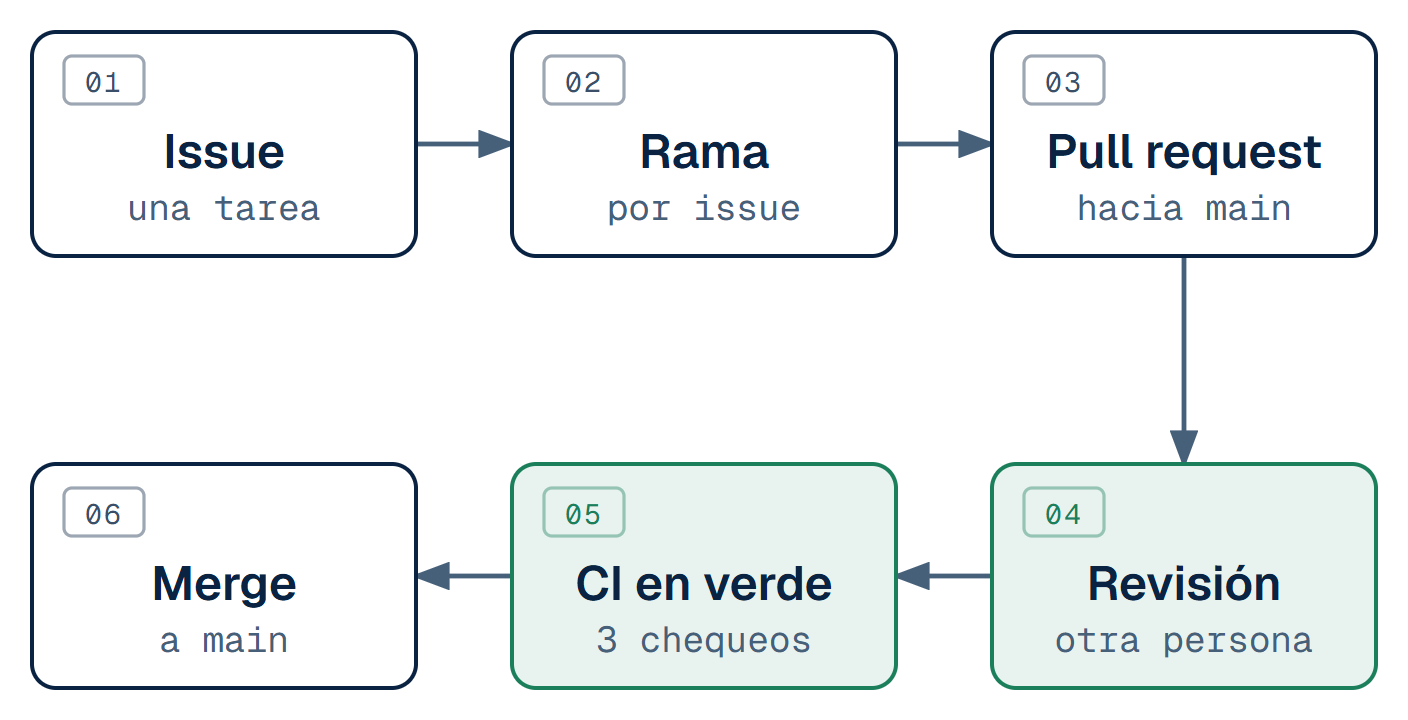
\includegraphics[width=\linewidth]{diagramas/cabal-flujo.png}}{Figura 1. Flujo de trabajo de cada cambio.}

  \separa
  \textbf{Etapas}
  \begin{itemize}
    \item \textbf{M1:} entrevistas, MVP, modelos y esquema SQL.
    \item \textbf{M2:} catálogo y formulario de producto.
    \item \textbf{M3:} ventas, historial con filtro y CI.
    \item \textbf{M4:} deshacer y archivar, tema de color, cierre del día,
      búsqueda y mejoras de Vender.
  \end{itemize}
  }
}

\block{TECNOLOGÍAS UTILIZADAS}{
  \textoposter
  \centrado{110pt}{%
  \begin{center}
    \textbf{Tabla 1. Tecnologías utilizadas}

    \vspace{4mm}
    \textotabla
    \begin{tabular}{ll}
      \toprule
      \textbf{Elemento} & \textbf{Versión} \\
      \midrule
      Flutter (SDK) & 3.47.5 \\
      Riverpod (estado) & 2.6.1 \\
      sqflite (SQLite) & 2.4.1 \\
      image\_picker (fotos) & 1.2.4 \\
      path\_provider (archivos) & 2.1.6 \\
      sqflite\_common\_ffi (pruebas) & 2.4.3 \\
      flutter\_lints (calidad) & 6.0.0 \\
      GitHub Actions (CI) & --- \\
      \bottomrule
    \end{tabular}
  \end{center}
  }
}

\block{RESUMEN CUANTITATIVO}{
  \textoposter
  \centrado{150pt}{%
  Trabajo integrado en \texttt{main} al 12 de noviembre de 2026.

  \vspace{4mm}
  \begin{center}
    \textbf{Tabla 2. Indicadores del proyecto}

    \vspace{4mm}
    \textotabla
    \begin{tabular}{lr}
      \toprule
      \textbf{Indicador} & \textbf{Valor} \\
      \midrule
      Integrantes & 5 \\
      Entrevistas a tenderos & 4 \\
      Issues cerrados & 55 \\
      Pull requests integrados & 62 \\
      Commits en \texttt{main} & 228 \\
      Pruebas automáticas & \pruebasN \\
      Tablas en la base de datos & 5 \\
      Pantallas & 10 \\
      Providers de Riverpod & 8 \\
      Servicios & 4 \\
      \bottomrule
    \end{tabular}
  \end{center}
  }
}

% ==========================================
% COLUMNA 3
% ==========================================
\column{0.33}

\block{RESULTADOS}{
  \textoposter
  \centrado{\dimexpr\sobrante+0mm\relax}{%
  \begin{itemize}
    \item El flujo funciona de punta a punta: catálogo, venta, historial y
      cierre del día.
    \item Los datos siguen ahí al cerrar la app, porque se guardan en SQLite.
    \item Cada venta guarda el precio de ese momento, así que cambiar un precio
      no altera las ventas anteriores.
    \item Un producto se borra deslizando y se recupera con \textit{Deshacer}.
      Si ya tiene ventas, se archiva.
  \end{itemize}

  \vspace{4mm}
  \figura{12.6cm}{\imagenopcional{width=\linewidth,height=10cm,keepaspectratio}{../evidencia-tema-de-color/hoja-de-cantidad-vender-ventas-cierre.png}}{Figura 2. Pantallas Vender, Ventas y Cierre del día.}
  }
}

\block{ARQUITECTURA DEL SISTEMA}{
  \textoposter
  \centrado{\dimexpr\sobrante+0mm\relax}{%
  \figura{17.5cm}{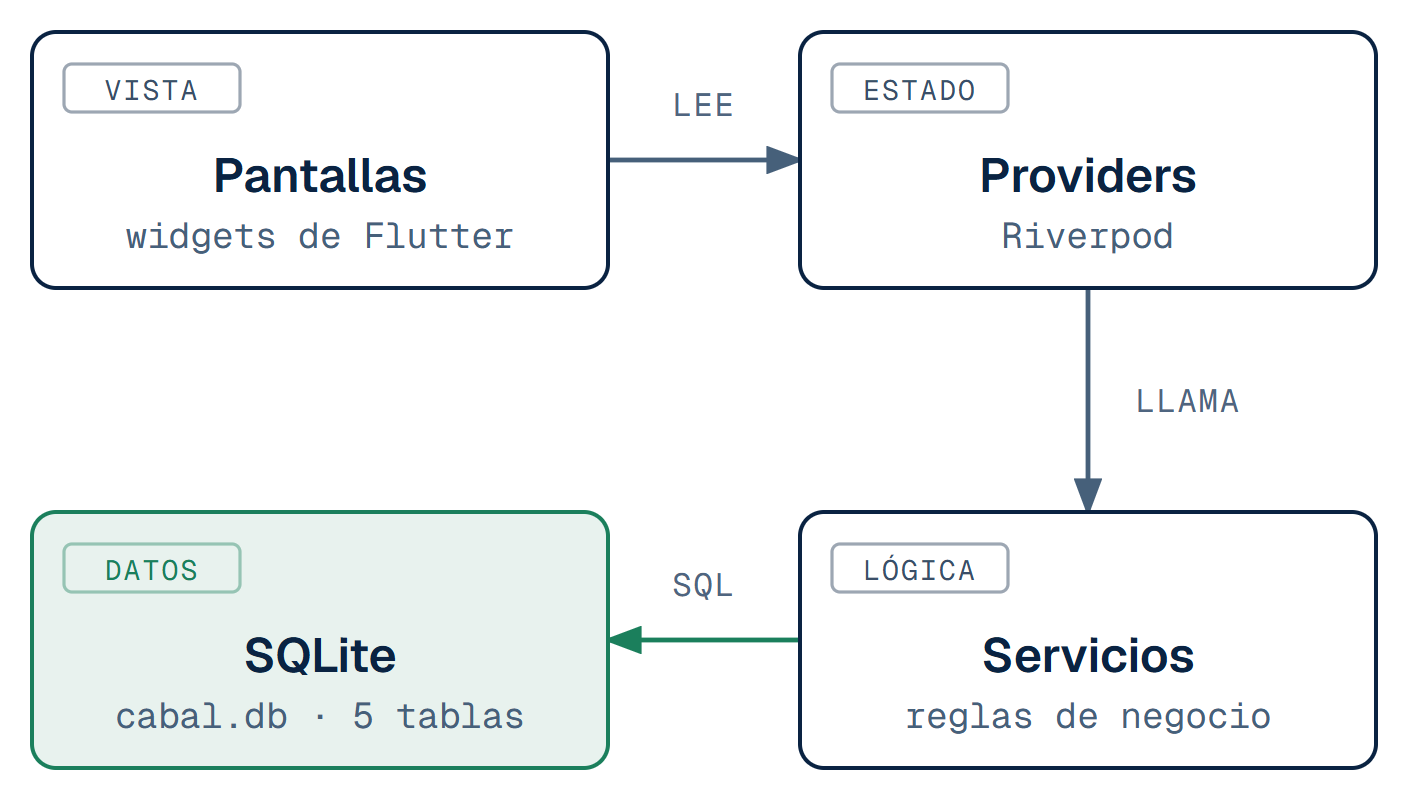
\includegraphics[width=\linewidth]{diagramas/cabal-arquitectura.png}}{Figura 3. Solo los servicios usan SQLite. Cada venta se guarda en una transacción: completa o no se guarda.}
  }
}

\block{REFERENCIAS}{
  \textoreferencias
  \centrado{0mm}{%
  \renewcommand{\bibsection}{}\setlength{\bibsep}{3mm}
  \begin{thebibliography}{9}
  \bibitem{riverpod} R. Rousselet, ``Riverpod,'' documentación oficial.
    \url{https://riverpod.dev}
  \bibitem{flutter} Google, ``Flutter documentation.''
    \url{https://docs.flutter.dev}
  \bibitem{sqflite} Tekartik, ``sqflite,'' paquete de SQLite para Flutter.
    \url{https://pub.dev/packages/sqflite}
  \bibitem{sqlite} D. R. Hipp, ``SQLite,'' documentación oficial.
    \url{https://www.sqlite.org}
  \bibitem{material} Google, ``Material Design 3.''
    \url{https://m3.material.io}
  \bibitem{progit} S. Chacon y B. Straub, \textit{Pro Git}, 2.ª ed. Apress, 2014.
  \bibitem{portigal} S. Portigal, \textit{Interviewing Users}. Rosenfeld Media,
    2013.
  \end{thebibliography}
  }
}

\block{AGRADECIMIENTOS}{
  \textoposter
  \centrado{0mm}{%
  Al \textbf{Ing. Saúl Calderón}, por el curso de Programación de Dispositivos
  Móviles, y al \textbf{Lic. Néstor Fernández}, por el curso de Mercadeo y
  Gerencia, que nos ayudó a ver el producto desde el lado del negocio. A los
  tenderos entrevistados y a la Universidad Mesoamericana, sede Quetzaltenango.
  }
}

\end{columns}

\end{document}
